\begin{frame}{Գրաֆների դեկարտյան արտադրյալ}{Սահմանում}
$G$ և $H$ գրաֆների $G\square H$ դեկարտյան արտադրյալը.
\begin{align*}
V(G \square H) &= V(G) \times V(H) \\
E(G \square H) &= \{(u_1,v_1)(u_2,v_2) : &(u_1=u_2 \text{ և } v_1v_2 \in E(H)) \text{ կամ } &\\ 
& &(v_1=v_2 \text{ և } u_1u_2 \in E(G) \}&
\end{align*}
\begin{figure}[t!]
    \centering
    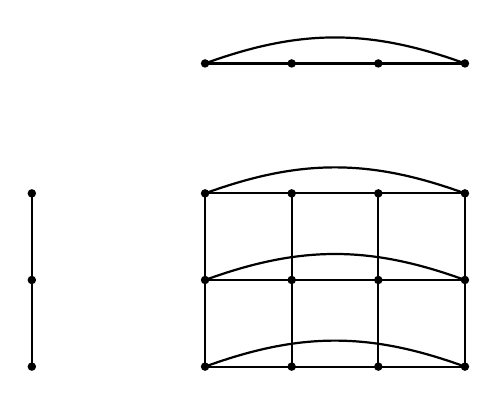
\begin{tikzpicture}[style=thick,scale=0.55, every node/.style={scale=0.55}]
        \coordinate (V11) at (0cm,2cm);
        \coordinate (V12) at (4cm,2cm);
        \coordinate (V13) at (6cm,2cm);
        \coordinate (V14) at (8cm,2cm);
        \coordinate (V15) at (10cm,2cm);
        \coordinate (V21) at (0cm,4cm);
        \coordinate (V22) at (4cm,4cm);
        \coordinate (V23) at (6cm,4cm);
        \coordinate (V24) at (8cm,4cm);
        \coordinate (V25) at (10cm,4cm);
        \coordinate (V31) at (0cm,6cm);
        \coordinate (V32) at (4cm,6cm);
        \coordinate (V33) at (6cm,6cm);
        \coordinate (V34) at (8cm,6cm);
        \coordinate (V35) at (10cm,6cm);
        \coordinate (V41) at (0cm,9cm);
        \coordinate (V42) at (4cm,9cm);
        \coordinate (V43) at (6cm,9cm);
        \coordinate (V44) at (8cm,9cm);
        \coordinate (V45) at (10cm,9cm);
        
        \draw<4-> (V12) -- (V13) -- (V14) -- (V15);
        \draw<4-> (V22) -- (V23) -- (V24) -- (V25);
        \draw<4-> (V32) -- (V33) -- (V34) -- (V35) ;
        \draw (V42) -- (V43) -- (V44) -- (V45) ;
        
        \draw (V11) -- (V21) -- (V31);
        \draw<3-> (V12) -- (V22) -- (V32);
        \draw<3-> (V13) -- (V23) -- (V33);
        \draw<3-> (V14) -- (V24) -- (V34);
        \draw<3-> (V15) -- (V25) -- (V35);
        
        \draw<4-> (V12) edge [bend left=20] (V15);
        \draw<4-> (V22) edge [bend left=20] (V25);
        \draw<4-> (V32) edge [bend left=20] (V35);
        \draw (V42) edge [bend left=20] (V45);
        
        \draw[fill=black] (V11) circle (2pt) ;
        \draw<2->[fill=black] (V12) circle (2pt) ;
        \draw<2->[fill=black] (V13) circle (2pt) ;
        \draw<2->[fill=black] (V14) circle (2pt) ;
        \draw<2->[fill=black] (V15) circle (2pt) ;
        \draw[fill=black] (V21) circle (2pt) ;
        \draw<2->[fill=black] (V22) circle (2pt) ;
        \draw<2->[fill=black] (V23) circle (2pt) ;
        \draw<2->[fill=black] (V24) circle (2pt) ;
        \draw<2->[fill=black] (V25) circle (2pt) ;
        \draw[fill=black] (V31) circle (2pt) ;
        \draw<2->[fill=black] (V32) circle (2pt) ;
        \draw<2->[fill=black] (V33) circle (2pt) ;
        \draw<2->[fill=black] (V34) circle (2pt) ;
        \draw<2->[fill=black] (V35) circle (2pt) ;
%         \draw[fill=black] (V41) circle (2pt) ;
        \draw[fill=black] (V42) circle (2pt) ;
        \draw[fill=black] (V43) circle (2pt) ;
        \draw[fill=black] (V44) circle (2pt) ;
        \draw[fill=black] (V45) circle (2pt) ;
    \end{tikzpicture}
    \end{figure}
    
\end{frame}



\begin{frame}{Գրաֆների դեկարտյան արտադրյալների միջակայքային ներկելիությունը}


Եթե $G,H\in \mathfrak{N}$, ապա $G\square H\in \mathfrak{N}$ (Գիառո, Կուբալ, 2004)

\begin{table}[h]
    \def\arraystretch{1.8}

    \centering
    \begin{tabular}{c|c|c}
         & $G \square H \in \mathfrak{N}$ & $G \square H \notin \mathfrak{N}$ \\
         \hline
        $G \in \mathfrak{N}$, $H \in \mathfrak{N}$ & $G=H=K_2$ & հնարավոր չէ \\
        $G \in \mathfrak{N}$, $H \notin \mathfrak{N}$ & $G=K_2$, $H=K_3$ & $G=$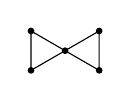
\begin{tikzpicture}[baseline=-0.5ex]
        \draw[fill=black] (0:0) circle(1pt);
        \draw[fill=black] (30:0.5cm) circle(1pt);
        \draw[fill=black] (-30:0.5cm) circle(1pt);
        \draw[fill=black] (150:0.5cm) circle(1pt);
        \draw[fill=black] (-150:0.5cm) circle(1pt);
        \draw (30:0.5cm) -- (0:0) -- (150:0.5cm) -- (-150:0.5cm) -- (0:0) -- (-30:0.5cm) -- cycle;
        \end{tikzpicture}, $H=K_3$ \\ 
        $G \notin \mathfrak{N}$, $H \notin \mathfrak{N}$ & $G=H=P_{10}$ & $G=H=K_3$ \\ 
        
    \end{tabular}
\end{table}
\end{frame}

